% =====================================================================
%  Kalender der FF KRZ -- Anleitung für Mitglieder
%  Vorlage: deb-support (debsupport.sty, siehe latex/README.md)
%  Übersetzen mit:  pdflatex anleitung_mitglieder_kalender_ff_krz.tex   (2x)
%  Bilder: Unterordner bilder/ (Screenshots des Web-Frontends)
% =====================================================================
\documentclass[a4paper,fontsize=10pt]{scrartcl}
\usepackage[bericht]{debsupport}
\usepackage{float}
\usepackage{needspace}

% Vor dem Verteilen anpassen:
\newcommand{\kalenderadresse}{kalender.example.de}   % endgültige Adresse des Kalenderservers
\newcommand{\hilfe}{die Betreuer des Kalenders (Kontakt siehe Aushang im Gerätehaus)}

\renewcommand*{\dsdokumentart}{Anleitung für Mitglieder}
\renewcommand*{\dskurztitel}{Kalender der FF KRZ -- Anleitung für Mitglieder}
\renewcommand*{\dsbeleg}{}
\setlength{\emergencystretch}{3em}
\graphicspath{{bilder/}}

% Bildschirmfoto mit dünnem Rahmen
\newcommand{\bild}[3][0.9\linewidth]{%
  \begin{figure}[H]\centering
    \fcolorbox{dsgrau!40}{white}{\includegraphics[width=#1]{#2}}
    \caption{#3}
  \end{figure}}
\newcommand{\knopf}[1]{\textsf{\textbf{#1}}}
% Warnkasten "Abonnieren, nicht importieren"; #1 = passende Menüpunkte
\newcommand{\nichtimportieren}[1]{%
  \begin{dshinweis}[title={Wichtig: abonnieren -- nicht importieren}]
  Nur ein \textbf{Abo} hält die Termine aktuell. Wird der Kalender
  \textbf{importiert}, werden die Termine einmalig kopiert: Änderungen und
  Absagen kommen danach nicht mehr an, und bei einem zweiten Import entstehen
  doppelte Termine.
  \begin{itemize}[leftmargin=1.2em]
    #1
    \item Den Abo-Link \textbf{nicht im Browser öffnen oder antippen} und
          keine \texttt{.ics}-Datei herunterladen und öffnen -- das wäre ein
          Import.
  \end{itemize}
  \textbf{So erkennen Sie ein Abo:} Der Kalender steht unter
  \glqq Abonnierte Kalender\grqq\ bzw.\ \glqq Weitere Kalender\grqq, und die
  Termine lassen sich nicht bearbeiten.
  \end{dshinweis}}
\newcommand{\menue}[1]{\textsf{#1}}

\begin{document}

\dstitel{Kalender der FF KRZ}
        {Alle Termine automatisch auf Smartphone, Tablet und in Outlook}
        {Stand:     & \today\\
         Für:       & alle Mitglieder der FF KRZ\\
         Adresse:   & \texttt{\kalenderadresse}}

\tableofcontents

% ------------------------------------------------------------------
\section{Worum geht es?}

Unsere Termine -- Übungsdienste, Sitzungen, Lehrgänge, die
Jahreshauptversammlung -- werden in MP Feuer gepflegt. Bisher mussten Sie
dort selbst nachsehen oder die Termine von Hand in Ihren eigenen Kalender
übertragen. Verschob sich ein Termin oder fiel er aus, merkte man das oft
erst spät.

Mit dem \textbf{Kalender der FF KRZ} kommen die Termine jetzt
\textbf{automatisch} in den Kalender, den Sie ohnehin benutzen: auf dem
iPhone, dem Android-Smartphone, dem Tablet oder in Outlook. Sie richten das
einmal ein, danach läuft alles von selbst.

\subsection*{Was ist neu?}

\begin{itemize}
  \item \textbf{Ihre Termine kommen von selbst.} Sie sehen genau die Termine,
        die zu Ihren Einheiten, Gruppen, Abteilungen und Lehrgängen gehören --
        zum Beispiel \emph{LG Drove}, \emph{JF Gr1} oder \emph{TM1 2027}.
        Termine der gesamten Wehr (\emph{FF KRZ}) sieht jedes Mitglied.
  \item \textbf{Immer aktuell.} Wird ein Termin in MP Feuer geändert oder
        abgesagt, ändert er sich auch auf Ihrem Gerät. Abgesagte Termine
        stehen mit \glqq Abgesagt:\grqq\ vor dem Titel im Kalender.
  \item \textbf{Ein Kalender je Gruppe.} Jede Einheit und Gruppe hat einen
        eigenen Kalender mit eigener Farbe. Sie können einzelne Kalender in
        Ihrer Kalender-App ein- und ausblenden.
  \item \textbf{Auf allen Geräten.} iPhone, iPad, Android, Outlook (Windows,
        Mac, Web) und Google Kalender -- auf Android auch ganz ohne
        zusätzliche App. Ein Zugang reicht für beliebig viele Geräte.
  \item \textbf{Neue Gruppe, neuer Kalender.} Kommen Sie in MP Feuer in eine
        neue Gruppe oder einen Lehrgang, erscheint der passende Kalender
        automatisch auf Smartphone und Tablet. Sie erhalten dazu eine kurze
        E-Mail.
  \item \textbf{Jahresübersicht zum Ausdrucken.} Ein Jahreskalender mit allen
        Ihren Terminen als PDF, z.\,B.\ für den Kühlschrank (Abschnitt~\ref{sec:pdf}).
  \item \textbf{Nur lesend und sicher.} Termine werden weiterhin nur in
        MP Feuer gepflegt; auf den Geräten kann niemand versehentlich etwas
        ändern. Sie haben einen persönlichen Zugang, und Sie sehen nur Ihre
        eigenen Kalender.
\end{itemize}

\begin{dshinweis}[title={Das brauchen Sie}]
\begin{itemize}[leftmargin=1.2em]
  \item die \textbf{Begrüßungs-E-Mail} des Kalenders (sie kommt an die in
        MP Feuer hinterlegte E-Mail-Adresse),
  \item Ihr Smartphone, Tablet oder Ihren PC mit Outlook,
  \item etwa \textbf{10 Minuten} für die einmalige Einrichtung.
\end{itemize}
Keine E-Mail bekommen? Siehe \glqq Häufige Fragen\grqq\ (Abschnitt~\ref{sec:faq}).
\end{dshinweis}

% ------------------------------------------------------------------
\section{Erste Anmeldung}\label{sec:anmeldung}

\subsection*{Schritt 1: Begrüßungs-E-Mail öffnen}

Sie erhalten eine E-Mail \glqq Willkommen beim Kalender der FF KRZ\grqq.
Darin stehen Ihr \textbf{Benutzername} (Form \texttt{vorname.nachname},
Umlaute ausgeschrieben, z.\,B.\ \texttt{juergen.mueller}) und Ihre Kalender.
Klicken Sie auf \knopf{Jetzt anmelden}.

\bild[0.6\linewidth]{begruessung.png}{Die Begrüßungs-E-Mail}

Das Passwort steht bewusst \emph{nicht} in der E-Mail. Sie finden es nach
der Anmeldung im Web-Frontend.

\subsection*{Schritt 2: Anmeldung bestätigen}

Es öffnet sich eine Seite mit Ihrem Benutzernamen. Klicken Sie noch einmal
auf \knopf{Jetzt anmelden}. Danach sind Sie angemeldet und sehen Ihre
Startseite.

\bild[0.6\linewidth]{link-bestaetigen.png}{Anmeldung bestätigen}

\begin{dshinweis}[title={Gut zu wissen}]
Der Link in der E-Mail gilt \textbf{14 Tage} und nur \textbf{einmal}. Ist er
abgelaufen oder schon benutzt, fordern Sie auf der Anmeldeseite unter
\menue{Anmeldelink anfordern} einfach einen neuen an
(\texttt{\kalenderadresse/login/link}). Dieser gilt 30 Minuten.
\end{dshinweis}

\subsection*{Später: Anmelden mit Passwort}

Unter \texttt{\kalenderadresse} können Sie sich jederzeit mit
\textbf{Benutzername oder E-Mail-Adresse} und Ihrem \textbf{Passwort}
anmelden. Das Passwort finden Sie unter \menue{Kalender abonnieren}
$\rightarrow$ \menue{Smartphone \& Tablet} (Abschnitt~\ref{sec:geraete}).

\bild[0.55\linewidth]{login.png}{Die Anmeldeseite}

% ------------------------------------------------------------------
\section{Ihre Startseite: Meine Kalender}

Nach der Anmeldung sehen Sie, welche Kalender für Sie freigeschaltet sind --
jeweils mit Farbe, kurzer Beschreibung und der Zahl der Termine im laufenden
Jahr. Darunter steht klein, \emph{warum} Sie den Kalender sehen: aus welcher
Mitgliedschaft in MP Feuer er stammt (\glqq aus: LG Drove\grqq) oder dass er
\glqq für alle Mitglieder\grqq\ gilt. Sind Sie in MP Feuer in einer Gruppe,
für die es keinen eigenen Kalender gibt, steht das unter der Liste.

\bild[0.8\linewidth]{startseite.png}{Die Startseite}

Fehlt ein Kalender oder stimmt eine Mitgliedschaft nicht, muss das in
\textbf{MP Feuer} geändert werden. Nach dem nächsten Abgleich passt sich der
Kalender automatisch an.

Mit \knopf{Kalender abonnieren} geht es zur Einrichtung Ihrer Geräte. Oben
im Menü finden Sie:

\begin{description}[style=sameline, leftmargin=3.9cm, font=\sffamily\bfseries]
  \item[Meine Kalender] Ihre Kalender im Überblick, mit Herkunft
  \item[Kalender abonnieren] die Angaben für Smartphone und Tablet sowie die
        Abo-Links für Outlook und den Google Kalender
  \item[Terminübersicht] Jahreskalender als PDF
  \item[Anleitungen] die Einrichtungsschritte für alle Geräte, auch online
\end{description}

% ------------------------------------------------------------------
\section{Kalender abonnieren: Welcher Weg passt?}\label{sec:abonnieren}

Unter \menue{Kalender abonnieren} wählen Sie, wo die Termine erscheinen
sollen. Sie können beides gleichzeitig nutzen, z.\,B.\ auf dem Smartphone und
in Outlook.

\bild[0.75\linewidth]{abonnieren.png}{Kalender abonnieren}

\begin{center}
\begin{tabularx}{\linewidth}{>{\raggedright\arraybackslash}p{3.6cm}XX}
\toprule
 & \textbf{Smartphone \& Tablet} & \textbf{Outlook \& Google Kalender} \\
\midrule
Geräte & iPhone, iPad, Android (mit App DAVx\textsuperscript{5}) &
  Outlook (Windows, Mac, Web), Google Kalender -- auch auf Android ohne
  Zusatz-App \\
\addlinespace
Einrichtung & einmal mit Benutzername und Passwort, für \emph{alle}
  Kalender & je Kalender einen Abo-Link \\
\addlinespace
Neue Kalender & erscheinen automatisch & einmal zusätzlich abonnieren \\
\addlinespace
Aktualisierung & meist alle 15--60 Minuten & teils nur alle paar Stunden \\
\addlinespace
Abschnitt & \ref{sec:geraete} & \ref{sec:google} und \ref{sec:outlook} \\
\bottomrule
\end{tabularx}
\end{center}

% ------------------------------------------------------------------
\section{Smartphone und Tablet einrichten}\label{sec:geraete}

Unter \menue{Kalender abonnieren} $\rightarrow$ \menue{Smartphone \&
Tablet} stehen alle Angaben, die Ihr Gerät braucht. Das Passwort ist zunächst
verdeckt; mit \knopf{Passwort anzeigen} machen Sie es sichtbar, mit
\knopf{Kopieren} übernehmen Sie es in die Zwischenablage.

\bild[0.75\linewidth]{geraete.png}{Die Seite \glqq Smartphone \& Tablet\grqq}

Ein Zugang gilt für \textbf{alle} Ihre Kalender und für beliebig viele
Geräte. Unter \glqq Letzter Abruf\grqq\ sehen Sie später, ob Ihr Gerät
regelmäßig Termine abholt.

\needspace{0.45\textheight}
\subsection{iPhone und iPad}

\textbf{Am einfachsten mit dem Konfigurationsprofil:}

\noindent\begin{minipage}[t]{0.64\linewidth}
\begin{enumerate}
  \item Auf dem iPhone bzw.\ iPad in \textbf{Safari} \texttt{\kalenderadresse}
        öffnen und anmelden (Abschnitt~\ref{sec:anmeldung}).
  \item \menue{Kalender abonnieren} $\rightarrow$ \menue{Smartphone \&
        Tablet} öffnen und weiter unten auf \knopf{Profil für iPhone/iPad
        laden} tippen. Den Download \knopf{Erlauben}.
  \item Die App \menue{Einstellungen} öffnen. Ganz oben erscheint
        \menue{Profil geladen} -- antippen. (Falls nicht:
        \menue{Einstellungen} $\rightarrow$ \menue{Allgemein} $\rightarrow$
        \menue{VPN und Geräteverwaltung} $\rightarrow$ \menue{Kalender FF KRZ}.)
  \item \knopf{Installieren} tippen, den Gerätecode eingeben und noch zweimal
        \knopf{Installieren} bestätigen. Der Hinweis \glqq nicht
        signiert\grqq\ ist normal.
  \item Die \menue{Kalender}-App öffnen. Nach kurzer Zeit erscheinen unter
        \menue{Kalender} die Kalender der FF KRZ.
\end{enumerate}
\end{minipage}\hfill
\begin{minipage}[t]{0.32\linewidth}
  \vspace{0pt}\centering
  \fcolorbox{dsgrau!40}{white}{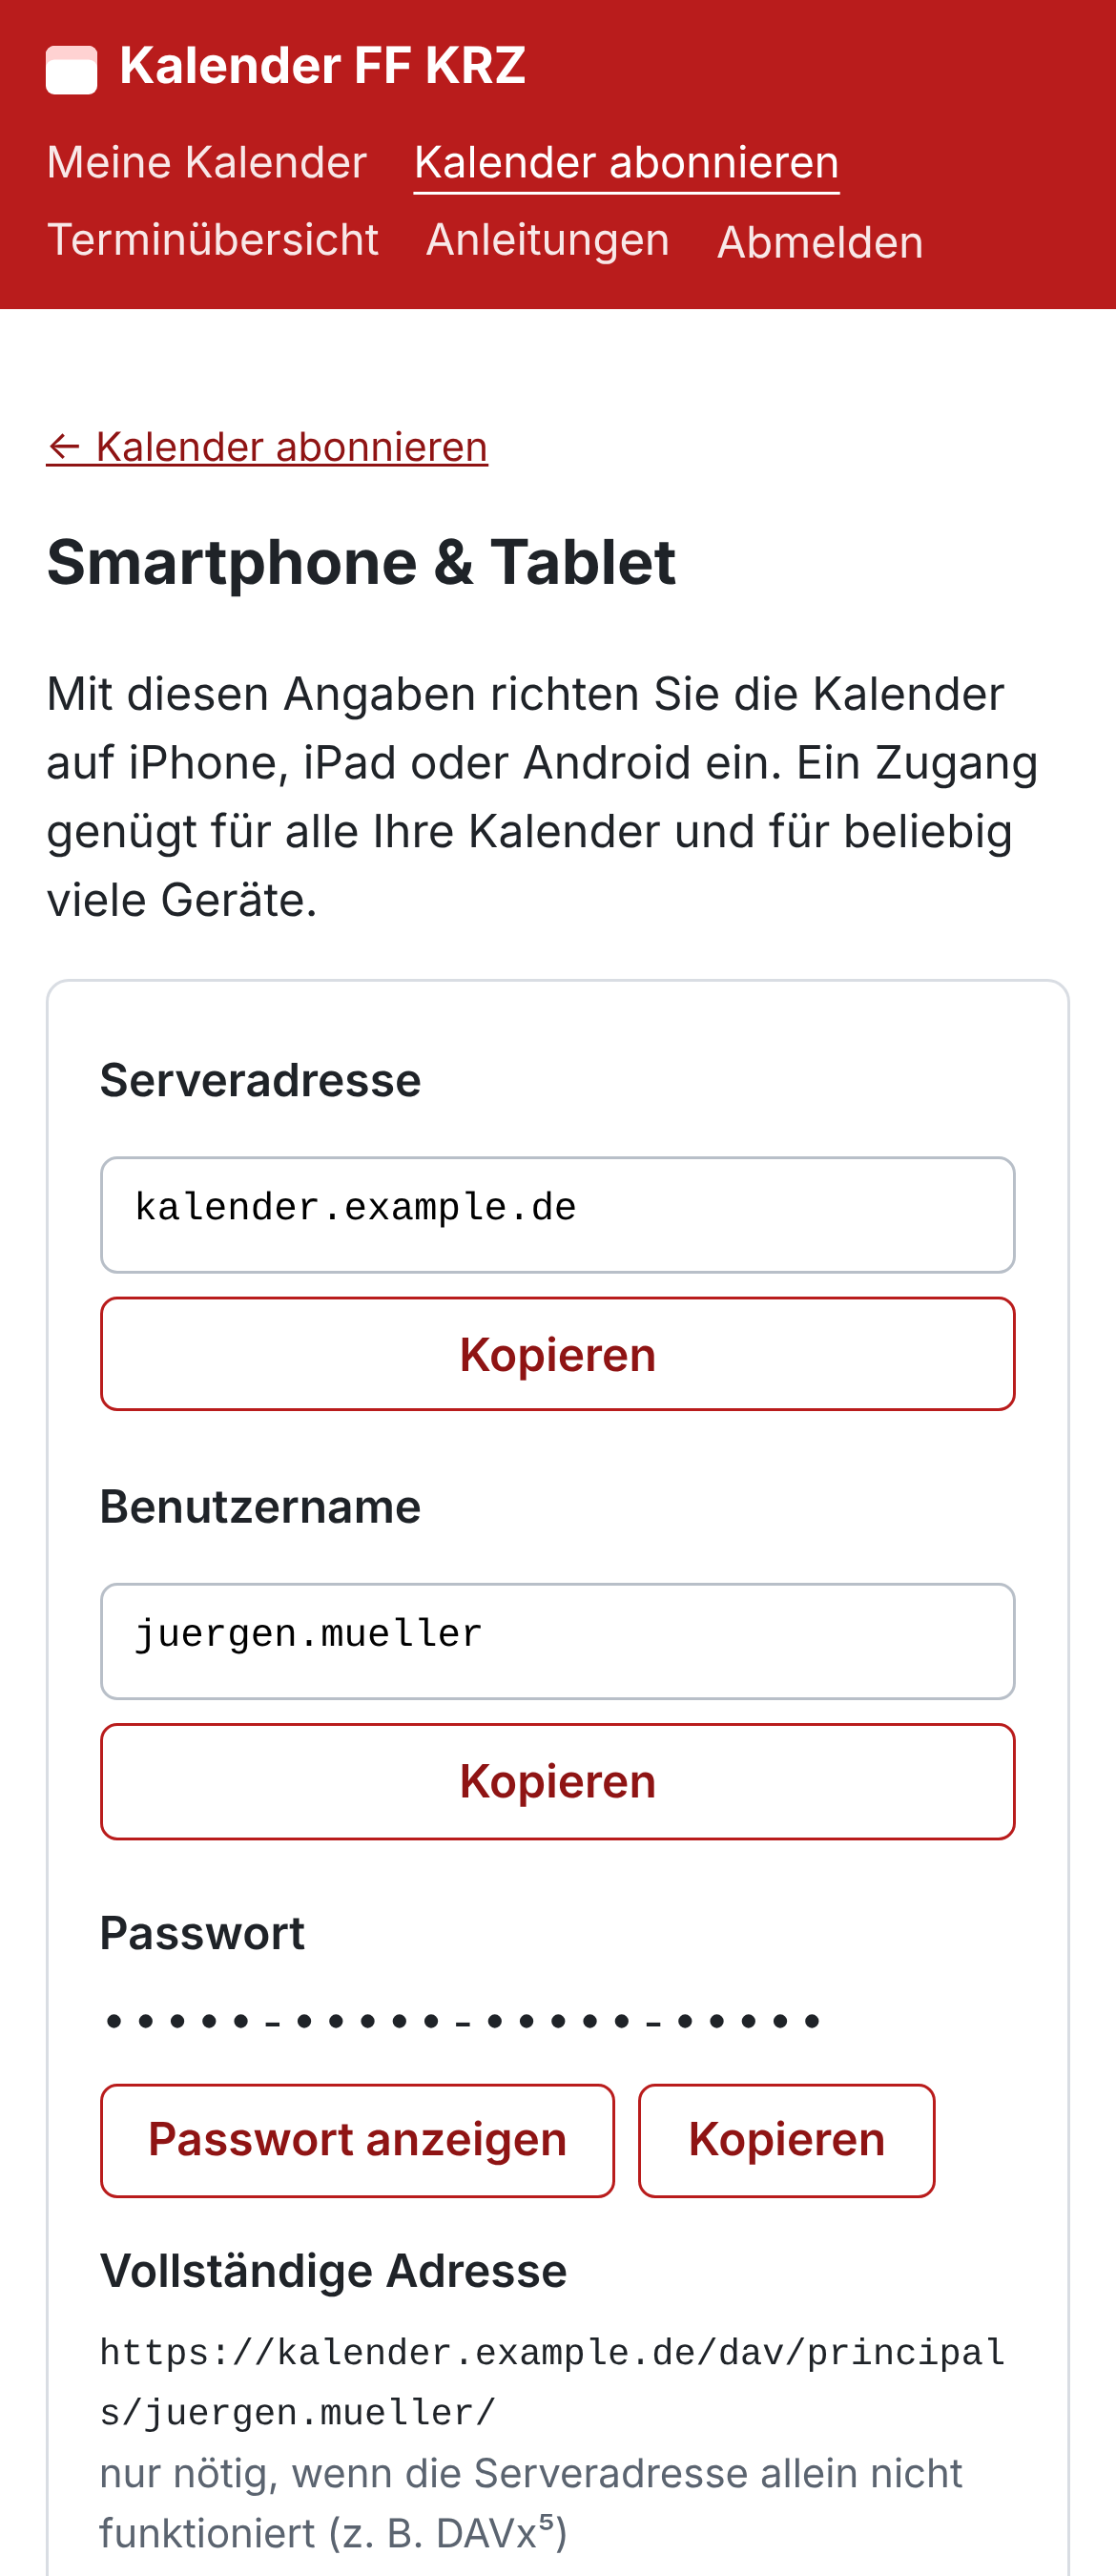
\includegraphics[width=0.85\linewidth]{handy-geraete-oben.png}}\\[2pt]
  {\small Die Seite auf dem iPhone}
\end{minipage}

\textbf{Oder von Hand einrichten:}

\begin{enumerate}
  \item \menue{Einstellungen} $\rightarrow$ \menue{Apps} $\rightarrow$
        \menue{Kalender} $\rightarrow$ \menue{Kalender-Accounts} $\rightarrow$
        \menue{Account hinzufügen} (ältere iOS-Versionen:
        \menue{Einstellungen} $\rightarrow$ \menue{Kalender} $\rightarrow$
        \menue{Accounts}).
  \item \menue{Andere} $\rightarrow$ \menue{CalDAV-Account hinzufügen}.
  \item Eintragen: \textbf{Server} \texttt{\kalenderadresse},
        \textbf{Benutzername} und \textbf{Passwort} von der Seite
        \menue{Smartphone \& Tablet}, \textbf{Beschreibung} z.\,B.\
        \glqq Kalender FF KRZ\grqq.
  \item \knopf{Weiter}, Kalender eingeschaltet lassen, \knopf{Sichern}.
\end{enumerate}

\textbf{Tipp:} Wie oft das iPhone nachschaut, stellen Sie unter
\menue{Einstellungen} $\rightarrow$ \menue{Apps} $\rightarrow$
\menue{Kalender} $\rightarrow$ \menue{Kalender-Accounts} $\rightarrow$
\menue{Datenabgleich} ein, z.\,B.\ \glqq Alle 15 Minuten\grqq.

\subsection{Android mit der App DAVx\textsuperscript{5}}

Android kann diese Kalender nicht von Haus aus abrufen. Dafür gibt es die App
\textbf{DAVx\textsuperscript{5}}. Einmal eingerichtet, erscheinen die
Kalender in \emph{jeder} Kalender-App, z.\,B.\ im Google Kalender oder Samsung
Kalender -- und bleiben genauso aktuell wie auf einem iPhone.

\begin{dshinweis}[title={Was kostet DAVx\textsuperscript{5}?}]
Im \textbf{Google Play Store} kostet die App \textbf{einmalig rund 5\,Euro}
(kein Abo). Ein Kauf gilt für alle Geräte mit demselben Google-Konto. Über den
alternativen App-Store \textbf{F-Droid} gibt es dieselbe App
\textbf{kostenlos}; dafür muss F-Droid aber erst selbst installiert werden.
Wer die App nicht möchte, nutzt den Weg über den Google Kalender
(Abschnitt~\ref{sec:google}).
\end{dshinweis}

\begin{enumerate}
  \item DAVx\textsuperscript{5} installieren und öffnen. Die Frage nach dem
        Zugriff auf Kalender mit \knopf{Zulassen} beantworten.
  \item Auf das \knopf{+} tippen und \menue{Mit URL und Benutzername
        anmelden} wählen.
  \item Eintragen: \textbf{Basis-URL} \texttt{https://\kalenderadresse},
        \textbf{Benutzername} und \textbf{Passwort} von der Seite
        \menue{Smartphone \& Tablet}. Klappt es nicht, als URL die
        \glqq Vollständige Adresse\grqq\ von derselben Seite verwenden.
  \item \knopf{Anmelden}, als Kontoname z.\,B.\ \glqq Kalender FF KRZ\grqq\
        eintragen und \knopf{Konto anlegen}.
  \item Im Konto den Reiter \menue{CalDAV} öffnen und die Kalender
        ankreuzen.
  \item In der Kalender-App ggf.\ die neuen Kalender einblenden (Google
        Kalender: Menü $\rightarrow$ Kalender des Kontos \glqq Kalender FF
        KRZ\grqq).
\end{enumerate}

\textbf{Tipps:} Unter DAVx\textsuperscript{5} $\rightarrow$ Konto
$\rightarrow$ Zahnrad stellen Sie das Synchronisationsintervall ein
(z.\,B.\ 15 oder 30 Minuten). Folgen Sie in DAVx\textsuperscript{5} dem Hinweis
zur \textbf{Akku-Optimierung} und schalten Sie sie für die App aus -- sonst
legt Android die App \glqq schlafen\grqq\ und es kommen keine Änderungen an.

% ------------------------------------------------------------------
\section{Android ohne Zusatz-App: über den Google Kalender}\label{sec:google}

Wer keine zusätzliche App installieren möchte, kann die Kalender auch im
\textbf{Google Kalender} abonnieren. Sie erscheinen dann in der
Google-Kalender-App auf dem Smartphone -- und auf allen anderen Geräten, die
mit demselben Google-Konto verbunden sind.

\begin{dshinweis}[title={Bitte vorher wissen}]
\begin{itemize}[leftmargin=1.2em]
  \item Google holt abonnierte Kalender nur \textbf{alle paar Stunden} ab,
        oft nur alle 8 bis 24 Stunden; das lässt sich nicht einstellen.
        Kurzfristige Änderungen und Absagen kommen deshalb spät an. Wer es
        aktuell braucht, nimmt DAVx\textsuperscript{5}
        (Abschnitt~\ref{sec:geraete}).
  \item Jeder Kalender wird \textbf{einzeln} abonniert. Kommt ein Kalender
        hinzu, erhalten Sie eine E-Mail und fügen den neuen Abo-Link einmal
        zusätzlich hinzu.
  \item Der Abo-Link ist persönlich und wird bei Google gespeichert. Bitte
        nicht weitergeben.
\end{itemize}
\end{dshinweis}

\nichtimportieren{\item Im Google Kalender \menue{Per URL} wählen --
  \emph{nicht} \menue{Importieren}.}

\textbf{Schritt 1 -- Abo-Link kopieren:} Unter \menue{Kalender abonnieren}
$\rightarrow$ \menue{Outlook \& Google Kalender} steht zu jedem Kalender
ein Abo-Link. Mit \knopf{Kopieren} übernehmen Sie ihn.

\bild[0.75\linewidth]{outlook-oben.png}{Abo-Links für Outlook und den Google Kalender (Ausschnitt)}

\textbf{Schritt 2 -- im Google Kalender hinzufügen:} Das geht nur im
Browser, nicht in der App. Am einfachsten am PC:

\begin{enumerate}
  \item \texttt{calendar.google.com} öffnen und mit dem Google-Konto anmelden,
        das auch auf dem Smartphone verwendet wird.
  \item Links neben \menue{Weitere Kalender} auf \knopf{+} klicken und
        \menue{Per URL} wählen.
  \item Den Abo-Link einfügen und \knopf{Kalender hinzufügen} klicken.
  \item Für jeden weiteren Kalender wiederholen.
\end{enumerate}

\textbf{Schritt 3 -- auf dem Smartphone einschalten:} In der
Google-Kalender-App Menü $\rightarrow$ \menue{Einstellungen} $\rightarrow$
den neuen Kalender antippen $\rightarrow$ \menue{Synchronisieren}
einschalten. Danach erscheinen die Termine -- beim ersten Mal kann das
einige Zeit dauern.

\textbf{Neue Abo-Links erzeugt?} Dann die alten Kalender im Google Kalender
entfernen (\menue{Einstellungen} $\rightarrow$ Kalender $\rightarrow$
\menue{Abo beenden}) und mit den neuen Links erneut hinzufügen.

% ------------------------------------------------------------------
\section{Outlook}\label{sec:outlook}

Auch Outlook verwendet die \textbf{Abo-Links} von der Seite
\menue{Kalender abonnieren} $\rightarrow$ \menue{Outlook \& Google
Kalender} (Abbildung in Abschnitt~\ref{sec:google}). Jeder Kalender wird einzeln
abonniert: Abo-Link mit \knopf{Kopieren} übernehmen, wie unten beschrieben
einfügen, für jeden weiteren Kalender wiederholen.

\nichtimportieren{\item In Outlook \menue{Aus dem Internet} bzw.\
  \menue{Internetkalender-Abonnement} wählen -- \emph{nicht}
  \menue{Aus Datei} oder \menue{Importieren}.}

\begin{dshinweis}[title={Bitte beachten}]
\begin{itemize}[leftmargin=1.2em]
  \item Der Abo-Link ist \textbf{persönlich und geheim}. Bitte nicht
        weitergeben.
  \item Outlook holt abonnierte Kalender seltener ab als ein Smartphone,
        teils nur alle paar Stunden. Für kurzfristige Absagen ist das
        Smartphone die bessere Quelle.
  \item Kommt ein neuer Kalender hinzu, erhalten Sie eine E-Mail. Den neuen
        Kalender bitte einmal zusätzlich abonnieren.
\end{itemize}
\end{dshinweis}

\subsection*{Outlook unter Windows (klassisch)}
\begin{enumerate}
  \item Abo-Link kopieren.
  \item In Outlook zur \menue{Kalender}-Ansicht wechseln.
  \item \menue{Start} $\rightarrow$ \menue{Kalender hinzufügen}
        $\rightarrow$ \menue{Aus dem Internet \ldots} (ältere Versionen:
        Rechtsklick auf \menue{Meine Kalender} $\rightarrow$
        \menue{Kalender hinzufügen} $\rightarrow$ \menue{Aus dem Internet}).
  \item Link einfügen, \knopf{OK} und die Rückfrage mit \knopf{Ja} bestätigen.
\end{enumerate}

\subsection*{Neues Outlook und Outlook im Web}
\begin{enumerate}
  \item Abo-Link kopieren.
  \item Im Kalender links auf \menue{Kalender hinzufügen} klicken.
  \item \menue{Aus dem Internet abonnieren} wählen.
  \item Link einfügen, Name und Farbe wählen, \knopf{Importieren}.
\end{enumerate}

\subsection*{Outlook für Mac}
\begin{enumerate}
  \item Abo-Link kopieren.
  \item \menue{Datei} $\rightarrow$ \menue{Neu} $\rightarrow$
        \menue{Internetkalender-Abonnement} (bzw.\ im Kalender:
        \menue{Kalender hinzufügen} $\rightarrow$ \menue{Aus dem Internet
        abonnieren}).
  \item Link einfügen und bestätigen.
\end{enumerate}

% ------------------------------------------------------------------
\section{Terminübersicht als PDF}\label{sec:pdf}

Unter \menue{Terminübersicht} erstellen Sie einen Jahreskalender mit Ihren
Terminen zum Ausdrucken -- z.\,B.\ für die Pinnwand oder den Kühlschrank.

\begin{enumerate}
  \item \textbf{Ab Monat} wählen (vorgegeben ist der Januar des laufenden
        Jahres) und den \textbf{Zeitraum} (1 bis 12 Monate).
  \item \textbf{Aufteilung}: alle Monate auf \emph{einer} Seite oder auf
        \emph{zwei} Seiten (z.\,B.\ Januar--Juni und Juli--Dezember) mit
        größeren Feldern.
  \item Die gewünschten \textbf{Kalender} ankreuzen.
  \item \knopf{PDF herunterladen}.
\end{enumerate}

\bild[0.6\linewidth]{terminuebersicht.png}{Auswahl für die Terminübersicht}

\bild{pdf-beispiel.png}{Beispiel: ein Jahr auf einer Seite}

\textbf{So lesen Sie den Jahreskalender:}

\begin{itemize}
  \item Jeder Termin ist ein farbiges Oval in der Farbe seines Kalenders,
        darin die \textbf{Startzeit}. Ein leeres Oval ist ein
        \textbf{ganztägiger} Termin.
  \item Ein \textbf{leerer Kreis mit farbigem Rand} ist ein
        \textbf{abgesagter} Termin.
  \item Sind an einem Tag zu viele Termine für Uhrzeiten, stehen dort nur
        farbige \textbf{Punkte}, ggf.\ mit \glqq +2\grqq\ für weitere.
  \item \textbf{Grau} sind Wochenenden und gesetzliche Feiertage in NRW, ein
        \textbf{blauer Streifen} am Rand markiert Schulferien in NRW.
  \item Titel und Orte stehen bewusst nicht im PDF. Was hinter einem Termin
        steckt, sehen Sie auf Ihrem Smartphone oder in Outlook.
  \item Das PDF zeigt den Stand beim Herunterladen (unten auf der Seite).
        Für spätere Änderungen einfach ein neues PDF erstellen.
\end{itemize}

% ------------------------------------------------------------------
\section{Häufige Fragen}\label{sec:faq}

\subsection*{Ich habe keine Begrüßungs-E-Mail bekommen.}
Sehen Sie bitte im Spam-Ordner nach. Ansonsten können Sie sich unter
\texttt{\kalenderadresse/login/link} jederzeit einen Anmeldelink schicken
lassen -- an die E-Mail-Adresse, die in MP Feuer hinterlegt ist. Kommt auch
dieser nicht an, ist in MP Feuer vermutlich keine oder eine falsche Adresse
eingetragen.

\subsection*{Ich habe mein Passwort vergessen.}
Lassen Sie sich unter \texttt{\kalenderadresse/login/link} einen Anmeldelink
schicken. Nach der Anmeldung steht Ihr Passwort unter \menue{Kalender
abonnieren} $\rightarrow$ \menue{Smartphone \& Tablet}.

\needspace{0.25\textheight}
\subsection*{Mein Handy ist weg, oder ich habe einen Abo-Link aus Versehen weitergegeben.}
Unter \menue{Kalender abonnieren} erzeugen Sie neue Zugangsdaten. Die alten
gelten dann sofort nicht mehr:
\begin{itemize}
  \item \textbf{Handy oder Tablet verloren:} auf der Seite \menue{Smartphone
        \& Tablet} unten \knopf{Neues Passwort \ldots}. Danach auf Ihren
        übrigen Geräten das neue Passwort eintragen. Outlook und der Google
        Kalender sind nicht betroffen.
  \item \textbf{Abo-Link weitergegeben:} auf der Seite \menue{Outlook \&
        Google Kalender} unten \knopf{Neue Abo-Links \ldots}. Danach in
        Outlook bzw.\ im Google Kalender die alten Abos entfernen und die
        neuen Links abonnieren. Smartphone und Tablet sind nicht betroffen.
\end{itemize}
Vor dem Erzeugen fragt das Web-Frontend noch einmal nach:

\bild[0.6\linewidth]{neues-passwort.png}{Rückfrage vor dem neuen Passwort}

\subsection*{Ein Kalender fehlt -- oder ich sehe einen, den ich nicht brauche.}
Welche Kalender Sie sehen, ergibt sich aus Ihren Mitgliedschaften in
MP Feuer; auf der Startseite steht bei jedem Kalender, woher er kommt. Stimmt
dort etwas nicht, wenden
Sie sich an Ihre Einheitsführung bzw.\ an \hilfe. Einen Kalender, den Sie
nicht sehen möchten, können Sie in Ihrer Kalender-App einfach ausblenden.

\subsection*{Ich kann einen Termin nicht ändern oder löschen.}
Das ist so gewollt: Die Kalender sind nur lesend. Termine werden
ausschließlich in MP Feuer gepflegt. Eigene Termine legen Sie bitte in einem
Ihrer persönlichen Kalender an, nicht in den Kalendern der FF KRZ.

\subsection*{Eine Änderung ist noch nicht auf meinem Gerät.}
Änderungen erscheinen nach dem nächsten Abgleich mit MP Feuer und dem
nächsten Abruf durch Ihr Gerät. Smartphones holen meist alle 15 bis 60
Minuten ab, Outlook und Google teils nur alle paar Stunden. Auf der Seite
\menue{Kalender abonnieren} sehen Sie bei \menue{Smartphone \& Tablet} bzw.\
bei jedem Abo-Link, wann zuletzt erfolgreich abgerufen wurde.

\subsection*{Ich habe den Kalender aus Versehen importiert statt abonniert.}
Das merken Sie daran, dass Änderungen und Absagen nicht ankommen oder Termine
doppelt erscheinen. Löschen Sie die importierten Termine bzw.\ den importierten
Kalender und abonnieren Sie den Kalender neu, wie in
Abschnitt~\ref{sec:google} bzw.\ \ref{sec:outlook} beschrieben. Auf iPhone,
iPad und mit DAVx\textsuperscript{5} kann das nicht passieren, weil dort
Benutzername und Passwort verwendet werden.

\subsection*{Ich habe ein neues Handy.}
Einfach wie in Abschnitt~\ref{sec:geraete} neu einrichten -- mit demselben
Benutzernamen und Passwort.

\subsection*{Mein Name hat sich geändert.}
Ihr Zugang funktioniert unverändert weiter. Passt der Benutzername nicht mehr
zu Ihrem Namen, sehen Sie auf der Startseite einen Hinweis und können ihn
dort umstellen. Danach müssen Sie Smartphone und Tablet einmal mit dem neuen
Benutzernamen einrichten; Outlook läuft ohne Änderung weiter. Sie können den
alten Benutzernamen aber auch einfach behalten.

\subsection*{Mehrere aus unserer Familie haben dieselbe E-Mail-Adresse.}
Kein Problem: Jedes Mitglied hat einen eigenen Zugang mit eigenem
Benutzernamen und Passwort. Bei der Anmeldung mit der E-Mail-Adresse
entscheidet das Passwort, welcher Zugang geöffnet wird. Ein angeforderter
Anmeldelink kommt für jedes Mitglied als eigene E-Mail.

\subsection*{Die Anmeldung ist gesperrt.}
Nach zu vielen falschen Eingaben wird die Anmeldung für bis zu eine Stunde
gesperrt. Warten Sie kurz oder lassen Sie sich einen Anmeldelink schicken.
Lautet der Hinweis, Ihre E-Mail-Adresse sei ungültig, muss die Adresse in
MP Feuer korrigiert werden; danach funktioniert Ihr Zugang wieder wie vorher.

% ------------------------------------------------------------------
\section{Datenschutz und Hilfe}

Der Kalender speichert nur Ihren Namen, Ihre E-Mail-Adresse, Ihre
Mitgliedschaften und Ihre Termine sowie, wann Sie sich zuletzt angemeldet und
wann Ihre Geräte zuletzt abgerufen haben (mit Gerätetyp). Ihr Passwort wird
nie per E-Mail verschickt. Welche Termine jemand sieht, ergibt sich allein aus
den Mitgliedschaften in MP Feuer; die Betreuer des Kalenders sehen in der
Verwaltung keine Termininhalte. Scheiden Sie aus der
Feuerwehr aus, werden Ihr Zugang und alle Ihre Daten automatisch gelöscht.
Einzelheiten stehen im Web-Frontend unter \menue{Datenschutz}.

\begin{dshinweis}[title={Fragen oder Probleme?}]
Die Anleitungen finden Sie auch online unter \menue{Anleitungen} im
Web-Frontend. Kommen Sie nicht weiter, wenden Sie sich an \hilfe.
\end{dshinweis}

\end{document}
